%%%%%%%%%%%%%%%%%%%%%%%%%%%%%%%%%%%%%%%%%%%%%%%%%%%%%%%%%%%%%%%%%%%%%%%%
% A0 Conference Poster — Deep Hedging (NeurIPS-quality)
% Author: Pratham Kailasiya, IIT Roorkee
% Layout: A0 Portrait, 2-column × 3-row balanced grid
%%%%%%%%%%%%%%%%%%%%%%%%%%%%%%%%%%%%%%%%%%%%%%%%%%%%%%%%%%%%%%%%%%%%%%%%
\documentclass[25pt, a0paper, portrait]{tikzposter}

\usepackage[utf8]{inputenc}
\usepackage[T1]{fontenc}
\usepackage{helvet}
\renewcommand{\familydefault}{\sfdefault}
\usepackage{amsmath,amssymb}
\usepackage{mathtools}
\usepackage{booktabs}
\usepackage{enumitem}
\usepackage{graphicx}
\usepackage{pifont}
\usepackage{xcolor}
\usepackage{tikz}
\usetikzlibrary{shapes.geometric,arrows.meta,positioning,fit,calc,
                 decorations.pathreplacing,backgrounds}
\usepackage{pgfplots}
\pgfplotsset{compat=1.17}

% ── Math shortcuts ──
\newcommand{\E}{\mathbb{E}}
\newcommand{\R}{\mathbb{R}}
\newcommand{\PP}{\mathbb{P}}
\newcommand{\QQ}{\mathbb{Q}}
\newcommand{\cvar}{\mathrm{CVaR}}
\newcommand{\VaR}{\mathrm{VaR}}
\DeclareMathOperator*{\argmin}{arg\,min}

% ══════════════════════════════════════════════════════════════════════
% COLOR PALETTE — Professional, subtle, NeurIPS-inspired
% ══════════════════════════════════════════════════════════════════════
\definecolor{PosterBG}{HTML}{FFFFFF}
\definecolor{BlockBG}{HTML}{FFFFFF}
\definecolor{NavyPri}{HTML}{1F3B63}
\definecolor{SlateSecond}{HTML}{64748B}
\definecolor{AccWarm}{HTML}{E8913A}
\definecolor{SoftBlue}{HTML}{2E8BC0}
\definecolor{LightBG}{HTML}{F7F8F9}
\definecolor{TextDark}{HTML}{1E293B}
\definecolor{TextBody}{HTML}{334155}
\definecolor{RuleGray}{HTML}{CBD5E1}
\definecolor{GreenOK}{HTML}{16A34A}

% ── tikzposter theme: no visible borders, clean blocks ──
\definecolorstyle{NeurIPSClean}{
  \colorlet{colorOne}{NavyPri}
  \colorlet{colorTwo}{SoftBlue}
  \colorlet{colorThree}{BlockBG}
}{
  \colorlet{blocktitlebgcolor}{NavyPri}
  \colorlet{blocktitlefgcolor}{white}
  \colorlet{blockbodybgcolor}{BlockBG}
  \colorlet{blockbodyfgcolor}{TextBody}
  \colorlet{backgroundcolor}{PosterBG}
  \colorlet{framecolor}{PosterBG}
}

\usetheme{Default}
\usecolorstyle{NeurIPSClean}
\useblockstyle[roundedcorners=6]{Default}
\usetitlestyle{Default}

% ── Title ──
\title{\parbox{0.92\linewidth}{\centering
{\fontsize{82}{96}\selectfont\bfseries\color{NavyPri}%
Deep Hedging with Distributionally Robust,\\[6pt]
Curriculum, and Regime-Adaptive Neural Networks}}}
\author{{\fontsize{36}{44}\selectfont\bfseries Pratham Kailasiya}%
\quad{\fontsize{28}{34}\selectfont $\cdot$\quad
Department of Management Studies, Indian Institute of Technology Roorkee%
\quad$\cdot$\quad\texttt{pratham@ms.iitr.ac.in}}}
\institute{}

% ══════════════════════════════════════════════════════════════════════
\begin{document}
\maketitle[width=0.97\textwidth,titletotopverticalspace=8mm]

% ════════════════════ ROW 1 ════════════════════
\begin{columns}

% ── Block 1: Introduction & Problem/Motivation ──
\column{0.48}
\block{\Large 1\;\; Introduction \& Motivation}{
\color{TextBody}
Classical delta hedging assumes known dynamics and continuous rebalancing---both
violated in practice.  \textbf{Deep hedging} learns hedging strategies directly
from simulated paths, but three critical gaps remain:

\bigskip
\begin{center}
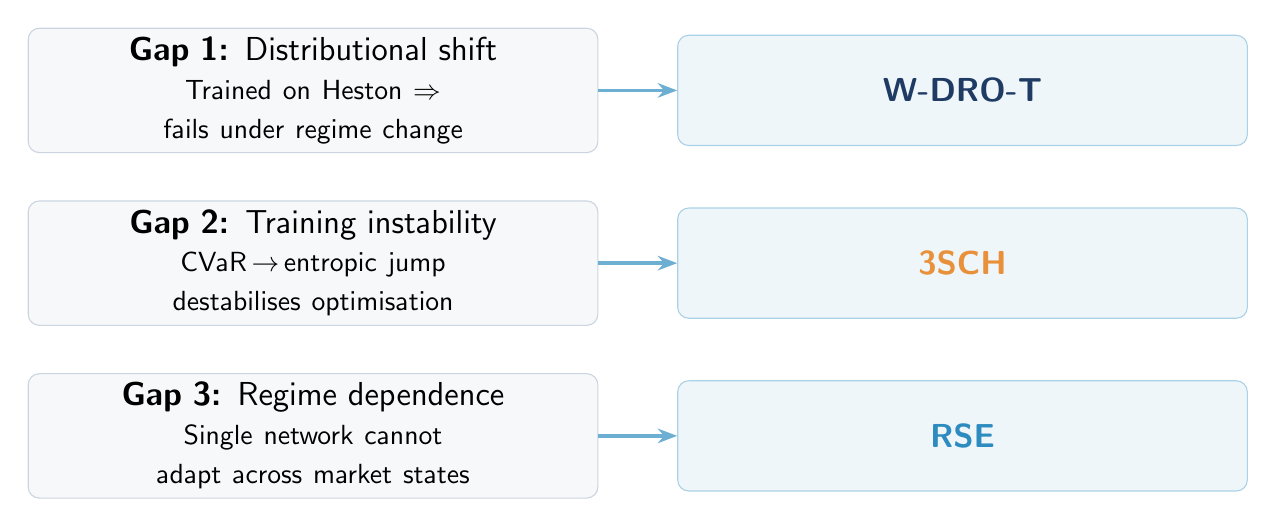
\begin{tikzpicture}[
  gap/.style={rectangle,rounded corners=4pt,draw=RuleGray,fill=LightBG,
              minimum height=14mm,text width=7cm,text centered,
              font=\large},
  sol/.style={rectangle,rounded corners=4pt,draw=SoftBlue!40,fill=SoftBlue!8,
              minimum height=14mm,text width=7cm,text centered,
              font=\large\bfseries},
  arr/.style={-{Stealth[length=7pt]},very thick,SoftBlue!70}]
\node[gap] (g1) {\textbf{Gap 1:} Distributional shift\\
  {\normalsize Trained on Heston $\Rightarrow$ fails under regime change}};
\node[gap,below=6mm of g1] (g2) {\textbf{Gap 2:} Training instability\\
  {\normalsize CVaR\,$\to$\,entropic jump destabilises optimisation}};
\node[gap,below=6mm of g2] (g3) {\textbf{Gap 3:} Regime dependence\\
  {\normalsize Single network cannot adapt across market states}};
\node[sol,right=10mm of g1] (s1) {\color{NavyPri}W-DRO-T};
\node[sol,right=10mm of g2] (s2) {\color{AccWarm}3SCH};
\node[sol,right=10mm of g3] (s3) {\color{SoftBlue}RSE};
\draw[arr] (g1) -- (s1);
\draw[arr] (g2) -- (s2);
\draw[arr] (g3) -- (s3);
\end{tikzpicture}
\end{center}

\bigskip
\textbf{Experimental protocol:}\;
80\,K Heston paths, $N\!=\!30$ steps, 10 seeds (42\,...\,942),
10\,K bootstrap, Holm--Bonferroni at $\alpha\!=\!0.05$, Cohen's $d$ effect sizes.
Real-market validation on SPY and NIFTY\,50 under normal, COVID-19, and GFC-2008 regimes.
}

% ── Block 2: Mathematical Formulation & Prior Work ──
\column{0.48}
\block{\Large 2\;\; Mathematical Formulation}{
\color{TextBody}
\textbf{\color{NavyPri}Heston stochastic-volatility model}
\vspace{-2pt}
\begin{align*}
dS_t &= rS_t\,dt + \sqrt{v_t}\,S_t\,dW^S_t \\[-2pt]
dv_t &= \kappa(\theta_v - v_t)\,dt + \xi\sqrt{v_t}\,dW^v_t,
\quad dW^S \!\cdot\! dW^v = \rho\,dt
\end{align*}

\textbf{\color{NavyPri}Deep hedging objective}\;
with P\&L\;
$\Pi(\delta)\!=\!{-Z}+\sum_k \delta_k\Delta S_k - c_{\mathrm{tc}}\sum_k|\delta_k-\delta_{k-1}|S_k$:
\vspace{-4pt}
\[
\theta^{*} = \argmin_\theta\;\rho\!\bigl(\Pi(\delta^\theta)\bigr)
\]

\medskip
\textbf{\color{NavyPri}Three novel risk objectives}

\smallskip
\tikz[baseline=-3pt]\draw[NavyPri,very thick](0,0)--(0.4,0);\;
\textbf{W-DRO-T}\; --- Wasserstein DRO with gradient-penalty dual:
\vspace{-6pt}
\[
\mathcal{L}_{\mathrm{DRO}}
 = \E_\PP[\ell(\theta;X)]
 + \varepsilon\,\E_\PP\!\bigl[\|\nabla_{\!X}\ell\|_2\bigr],
 \quad \varepsilon\!:\,0\!\to\!\varepsilon_{\max}
\]

\smallskip
\tikz[baseline=-3pt]\draw[AccWarm,very thick](0,0)--(0.4,0);\;
\textbf{3SCH}\; --- Three-stage curriculum homotopy:
\vspace{-6pt}
\[
\mathcal{L}_{\mathrm{mix}}(\alpha)
 = \alpha\,\cvar_{0.95}
 + (1\!-\!\alpha)\,\rho_\lambda^{\mathrm{ent}},
 \quad \alpha\!:\,0.8 \!\to\! 0.2
\]

\smallskip
\tikz[baseline=-3pt]\draw[SoftBlue,very thick](0,0)--(0.4,0);\;
\textbf{RSE}\; --- Regime-switching ensemble with gating:
\vspace{-6pt}
\[
\delta_k^{\mathrm{RSE}}
 = \textstyle\sum_{m=1}^{3} w_m(r_k)\,\delta_k^{(m)},\;\;
 w_m = \textstyle\sum_j p_j\bigl[\mathrm{softmax}(A/\tau)\bigr]_{jm}
\]

\medskip
{\small\color{SlateSecond}
\textbf{Prior work:}
Buehler et al.\ (2019) introduced deep hedging with CVaR.
We extend via distributional robustness (Sinha et al., 2018),
curriculum learning (Bengio et al., 2009), and ensemble methods (Lakshminarayanan et al., 2017).}
}

\end{columns}

% ════════════════════ ROW 2 ════════════════════
\begin{columns}

% ── Block 3: Method Overview / Novelty ──
\column{0.48}
\block{\Large 3\;\; Method Overview \& Novelty}{
\color{TextBody}
\begin{center}

\begin{tikzpicture}[
    node distance=6mm and 4mm,
    bx/.style={rectangle,draw=RuleGray,rounded corners=4pt,
               minimum width=4.2cm,minimum height=12mm,
               text centered,font=\normalsize\bfseries,fill=#1},
    ar/.style={-{Stealth[length=6pt]},thick,SlateSecond!70}]
\node[bx=LightBG]  (d) {Heston Simulator\\[-1pt]{\small 80\,K paths, 5-dim $I_k$}};
\node[bx=SoftBlue!12,right=of d]  (t) {Training Protocol\\[-1pt]{\small CVaR $\!\to\!$ Entropic}};
\node[bx=NavyPri!10,right=of t]   (m) {7 Models $\times$ 10 Seeds\\[-1pt]{\small W-DRO-T, 3SCH, RSE, \ldots}};
\node[bx=AccWarm!10,right=of m]   (b) {SPY + NIFTY\\[-1pt]{\small Backtest}};
\draw[ar](d)--(t); \draw[ar](t)--(m); \draw[ar](m)--(b);
\end{tikzpicture}
\end{center}

\medskip
\begin{minipage}[t]{0.48\linewidth}
\textbf{\color{NavyPri}W-DRO-T novelty}
\begin{itemize}[leftmargin=1em,itemsep=2pt,labelsep=0.3em,topsep=2pt]
\item[$\triangleright$] Gradient-penalty dual avoids inner
      sup over $\QQ$
\item[$\triangleright$] $\varepsilon$-annealing stabilises
      early training
\item[$\triangleright$] Transformer with causal mask +
      2\textsuperscript{nd}-order SDPA
\end{itemize}
\end{minipage}
\hfill
\begin{minipage}[t]{0.48\linewidth}
\textbf{\color{AccWarm}3SCH novelty}
\begin{itemize}[leftmargin=1em,itemsep=2pt,labelsep=0.3em,topsep=2pt]
\item[$\triangleright$] Mixed-loss convexity via Berge's
      maximum theorem
\item[$\triangleright$] Three-stage $\alpha$-annealing:
      warm-up, transition, fine-tune
\item[$\triangleright$] Zero-cost rollback to LSTM baseline
\end{itemize}
\end{minipage}

\medskip
\begin{minipage}[t]{0.48\linewidth}
\textbf{\color{SoftBlue}RSE novelty}
\begin{itemize}[leftmargin=1em,itemsep=2pt,labelsep=0.3em,topsep=2pt]
\item[$\triangleright$] Soft regime gating via learned
      affinity $A\!\in\!\R^{4\times3}$
\item[$\triangleright$] Regime features: realised vol, BiPV,
      returns, spread proxy
\item[$\triangleright$] Variance reduction:
      $\mathrm{Var}[\delta^{\mathrm{RSE}}] < \min_m \mathrm{Var}[\delta^{(m)}]$
\end{itemize}
\end{minipage}
\hfill
\begin{minipage}[t]{0.48\linewidth}
\textbf{\color{SlateSecond}Statistical rigour}
\begin{itemize}[leftmargin=1em,itemsep=2pt,labelsep=0.3em,topsep=2pt]
\item[$\triangleright$] 10\,000 bootstrap resamples for
      95\% CIs
\item[$\triangleright$] Paired $t$-tests with
      Holm--Bonferroni ($\alpha\!=\!0.05$)
\item[$\triangleright$] Cohen's $d$ effect size with
      magnitude classification
\end{itemize}
\end{minipage}
}

% ── Block 4: Key Results & Statistical Analysis ──
\column{0.48}
\block{\Large 4\;\; Key Results \& Statistical Analysis}{
\color{TextBody}
% --- CVaR bar chart ---
\begin{center}
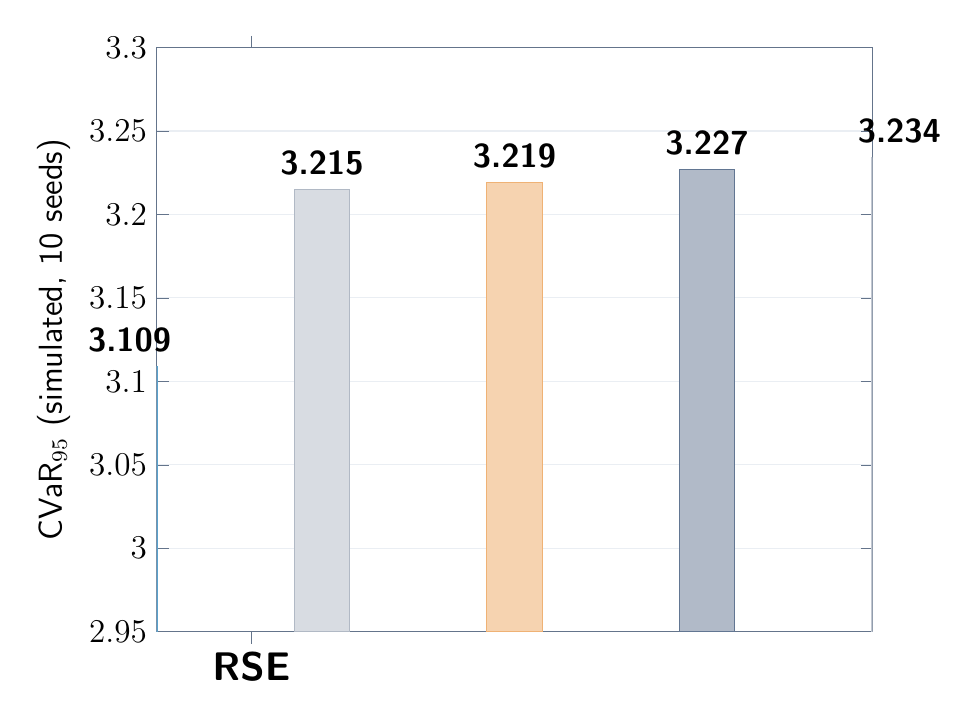
\begin{tikzpicture}
\begin{axis}[
    ybar, bar width=20pt,
    width=0.88\linewidth, height=9cm,
    symbolic x coords={RSE,LSTM,3SCH,W-DRO-T,Trans.},
    xtick=data,
    xticklabel style={font=\Large\bfseries},
    ymin=2.95, ymax=3.30,
    ylabel={\large CVaR$_{95}$ (simulated, 10 seeds)},
    ylabel style={font=\large},
    yticklabel style={font=\large},
    ymajorgrids=true,
    grid style={RuleGray!40},
    every node near coord/.append style={font=\large\bfseries,above=2pt},
    nodes near coords,
    nodes near coords align={vertical},
    point meta=explicit symbolic,
    enlarge x limits=0.18,
    axis line style={SlateSecond},
    tick style={SlateSecond},
]
\addplot[fill=SoftBlue!45,draw=SoftBlue!80]
  coordinates {(RSE,3.109) [3.109]};
\addplot[fill=SlateSecond!25,draw=SlateSecond!50]
  coordinates {(LSTM,3.215) [3.215]};
\addplot[fill=AccWarm!40,draw=AccWarm!70]
  coordinates {(3SCH,3.219) [3.219]};
\addplot[fill=NavyPri!35,draw=NavyPri!70]
  coordinates {(W-DRO-T,3.227) [3.227]};
\addplot[fill=SlateSecond!15,draw=SlateSecond!40]
  coordinates {(Trans.,3.234) [3.234]};
\end{axis}
\end{tikzpicture}
\end{center}

\smallskip
% --- Compact results table ---
\begin{center}
\renewcommand{\arraystretch}{1.15}
\setlength{\tabcolsep}{4pt}
{\small
\begin{tabular}{@{}l c c c c@{}}
\toprule
\textbf{Model} & \textbf{CVaR$_{95}$} & \textbf{95\% CI}
  & \textbf{$p$ vs LSTM} & \textbf{Cohen's $d$}\\
\cmidrule(r){1-1}\cmidrule(lr){2-2}\cmidrule(lr){3-3}\cmidrule(lr){4-4}\cmidrule(l){5-5}
RSE        & $3.109 \pm 0.010$ & $[3.104,\,3.115]$ & $<\!0.0001$ & $-7.41$\\
LSTM       & $3.215 \pm 0.015$ & $[3.207,\,3.225]$ & ---         & ---\\
3SCH       & $3.219 \pm 0.016$ & $[3.210,\,3.229]$ & $0.58$      & $+0.19$\\
W-DRO-T    & $3.227 \pm 0.011$ & $[3.220,\,3.234]$ & $0.10$      & $+0.60$\\
\bottomrule
\end{tabular}}
\end{center}
\vspace{2pt}
{\small\color{SlateSecond}
\textbf{RSE} achieves lowest simulated CVaR$_{95}$ ($3.109\!\pm\!0.010$)
with non-overlapping CI vs all baselines ($p\!<\!0.0001$, $|d|\!=\!7.41$).
10 seeds $\times$ 10K bootstrap.}
}

\end{columns}

% ════════════════════ ROW 3 ════════════════════
\begin{columns}

% ── Block 5: Real Market Validation & Crisis Testing ──
\column{0.48}
\block{\Large 5\;\; Real Market Validation \& Crisis Testing}{
\color{TextBody}
% --- SPY crisis bar chart ---
\begin{center}
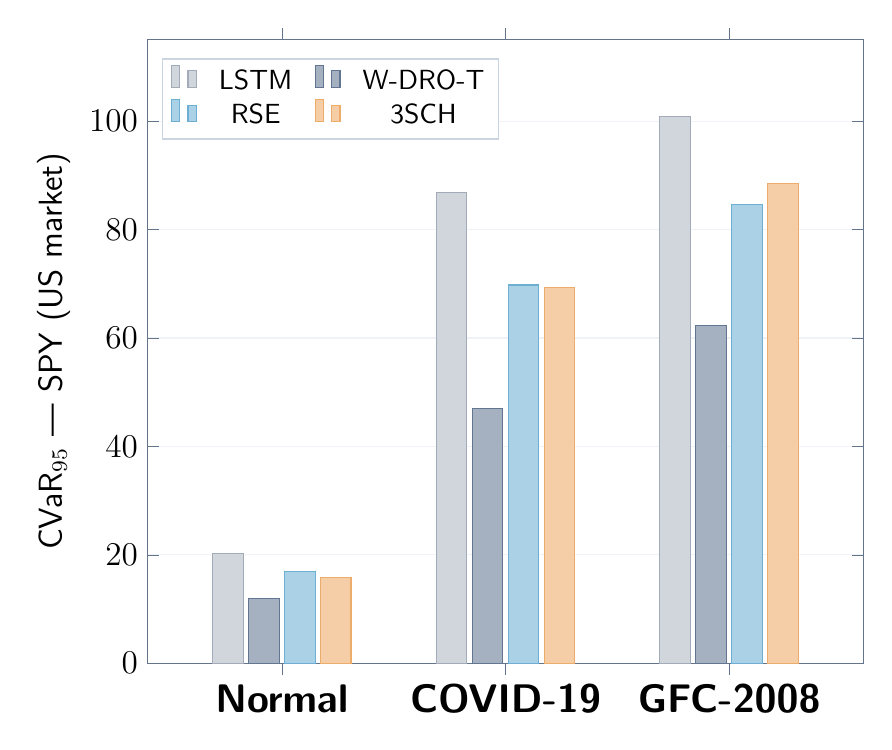
\begin{tikzpicture}
\begin{axis}[
    ybar, bar width=11pt,
    width=0.88\linewidth, height=9.5cm,
    symbolic x coords={Normal,COVID-19,GFC-2008},
    xtick=data,
    xticklabel style={font=\Large\bfseries},
    ymin=0, ymax=115,
    ylabel={\large CVaR$_{95}$ --- SPY (US market)},
    ylabel style={font=\large},
    yticklabel style={font=\large},
    ymajorgrids=true,
    grid style={RuleGray!30},
    legend style={at={(0.02,0.97)},anchor=north west,
                  font=\normalsize,draw=RuleGray,fill=white,
                  legend columns=2,column sep=6pt},
    enlarge x limits=0.30,
    axis line style={SlateSecond},
    tick style={SlateSecond},
]
\addplot[fill=SlateSecond!30,draw=SlateSecond!60]
  coordinates {(Normal,20.28) (COVID-19,86.84) (GFC-2008,100.88)};
\addplot[fill=NavyPri!40,draw=NavyPri!70]
  coordinates {(Normal,11.98) (COVID-19,46.94) (GFC-2008,62.26)};
\addplot[fill=SoftBlue!40,draw=SoftBlue!70]
  coordinates {(Normal,16.90) (COVID-19,69.76) (GFC-2008,84.57)};
\addplot[fill=AccWarm!45,draw=AccWarm!75]
  coordinates {(Normal,15.79) (COVID-19,69.25) (GFC-2008,88.43)};
\legend{LSTM,W-DRO-T,RSE,3SCH}
\end{axis}
\end{tikzpicture}
\end{center}

\smallskip
\begin{minipage}[t]{0.48\linewidth}
\textbf{\color{NavyPri}SPY (US, 5\,bps cost)}
\begin{itemize}[leftmargin=1em,itemsep=2pt,labelsep=0.3em,topsep=2pt]
\item[$\triangleright$] \textbf{W-DRO-T} dominates all scenarios
\item[$\triangleright$] Normal: $-41\%$ vs LSTM
\item[$\triangleright$] COVID-19: $-46\%$ vs LSTM
\item[$\triangleright$] GFC-2008: $-38\%$ vs LSTM
\item[$\triangleright$] Std P\&L: 1.71 (vs 5.05, $-66\%$)
\end{itemize}
\end{minipage}
\hfill
\begin{minipage}[t]{0.48\linewidth}
\textbf{\color{AccWarm}NIFTY\,50 (India, 18\,bps cost)}
\begin{itemize}[leftmargin=1em,itemsep=2pt,labelsep=0.3em,topsep=2pt]
\item[$\triangleright$] \textbf{3SCH} wins normal: CVaR\,=\,622
\item[$\triangleright$] \textbf{Transformer} wins COVID: 1644
\item[$\triangleright$] \textbf{W-DRO-T} wins GFC: 2350
\item[$\triangleright$] Higher vol (0.90) amplifies cost impact
\end{itemize}
\end{minipage}
}

% ── Block 6: Managerial, Regulatory, Risk & Deployment ──
\column{0.48}
\block{\Large 6\;\; Deployment, Risk \& Regulatory}{
\color{TextBody}
% --- Capital savings chart ---
\begin{center}
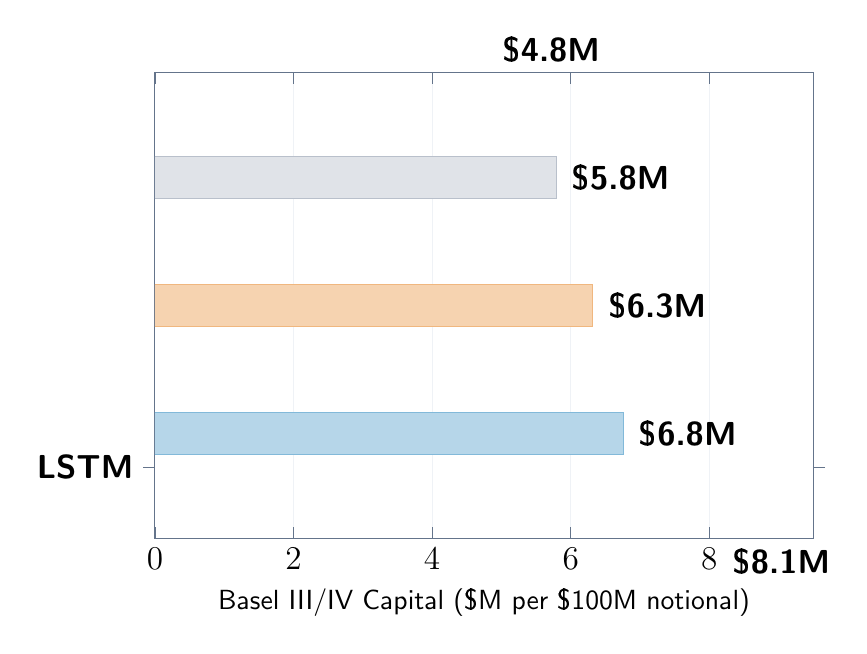
\begin{tikzpicture}
\begin{axis}[
    xbar, bar width=15pt,
    width=0.82\linewidth, height=7.5cm,
    symbolic y coords={LSTM,RSE,3SCH,Trans.,W-DRO-T},
    ytick=data,
    yticklabel style={font=\large\bfseries},
    xmin=0, xmax=9.5,
    xlabel={\normalsize Basel III/IV Capital (\$M per \$100M notional)},
    xlabel style={font=\normalsize},
    xticklabel style={font=\large},
    xmajorgrids=true,
    grid style={RuleGray!30},
    every node near coord/.append style={font=\large\bfseries,right=2pt},
    nodes near coords,
    nodes near coords align={horizontal},
    point meta=explicit symbolic,
    enlarge y limits=0.22,
    axis line style={SlateSecond},
    tick style={SlateSecond},
]
\addplot[fill=SlateSecond!30,draw=SlateSecond!60]
  coordinates {(8.11,LSTM) [\$8.1M]};
\addplot[fill=SoftBlue!35,draw=SoftBlue!60]
  coordinates {(6.76,RSE) [\$6.8M]};
\addplot[fill=AccWarm!40,draw=AccWarm!65]
  coordinates {(6.32,3SCH) [\$6.3M]};
\addplot[fill=SlateSecond!20,draw=SlateSecond!45]
  coordinates {(5.79,Trans.) [\$5.8M]};
\addplot[fill=NavyPri!45,draw=NavyPri!70]
  coordinates {(4.79,W-DRO-T) [\$4.8M]};
\end{axis}
\end{tikzpicture}
\end{center}

\smallskip
\begin{minipage}[t]{0.48\linewidth}
\textbf{\color{NavyPri}Deployment guidance}
\begin{itemize}[leftmargin=1em,itemsep=2pt,labelsep=0.3em,topsep=2pt]
\item[$\triangleright$] US capital: \textbf{W-DRO-T} ($-41\%$)
\item[$\triangleright$] India normal: \textbf{3SCH} (best CVaR)
\item[$\triangleright$] India crisis: \textbf{Transformer}
\item[$\triangleright$] Regime uncertainty: \textbf{RSE}
\item[$\triangleright$] \$10B desk: \$332M/yr freed capital
\end{itemize}
\end{minipage}
\hfill
\begin{minipage}[t]{0.48\linewidth}
\textbf{\color{NavyPri}Regulatory \& risk}
\begin{itemize}[leftmargin=1em,itemsep=2pt,labelsep=0.3em,topsep=2pt]
\item[\textcolor{GreenOK}{\ding{51}}] IFRS\,9 / Ind-AS\,109: 80--125\% offset
\item[\textcolor{GreenOK}{\ding{51}}] FRTB IMA: lower P\&L vol
\item[\textcolor{GreenOK}{\ding{51}}] SR\,11-7: RSE affinity interpretable
\item[\textcolor{GreenOK}{\ding{51}}] DRO degrades slower ($3.92\!\times$ vs $4.28\!\times$)
\end{itemize}
\end{minipage}

\bigskip
{\small\color{SlateSecond}
\textbf{Future work:}\;
Online adaptation \,$\to$\,
Multi-asset portfolios \,$\to$\,
Market impact models \,$\to$\,
Cross-market transfer \,$\to$\,
Hybrid 3SCH-DRO
\quad$\vert$\quad
\textbf{Code:} \texttt{github.com/pratham-kailasiya/deep-hedging}}
}

\end{columns}
\end{document}
